% Chapter 3

\chapter{引用与链接}

\section{脚注}
注释是对论文中特定名词或新名词的注解。注释可用页末注或篇末注的一种。选择页末注的应在注释与正文之间加细线分隔,线宽度为 1 点,线的长度不应超过纸张的三分之一宽度。同一页类列出多个注释的,应根据注释的先后顺序编排序号。字体为宋体5号,注释序号以“\circled{1}、\circled{2}”等数字形式标示在被注释词条的右上角。页末或篇末注释条目的序号应按照“\circled{1}、\circled{2}”等数字形式与被注释词条保持一致,脚注序号每面更新。示例:这里有个注释\footnote{我是解释注释的}。

\section{引用文中小节}\label{sec:ref}
如引用小节~\ref{sec:ref}

\section{引用参考文献}
这是一个参考文献引用的范例:BERT(Bidirectional Encoder Representations from Transformers)模型 \cite{devlin2018bert} 是由 Google AI 团队与 2018 年提出的语言表示模型,发布时在 NLP 领域的 11 个任务上取得了最好结果。经过微调后, BERT 可以灵活的应用在下游人物中。更多引用命令请参阅 natbib 文档或 biblatex 文档。\nocite{*}

文献引用需要配合 BibTeX 使用,很多工具可以直接生成 BibTeX 文件(如 EndNote、NoteExpress、百度学术、谷歌学术等),此处不作介绍。

\section{图片引用}

\begin{figure}[htbp]
    \centering
    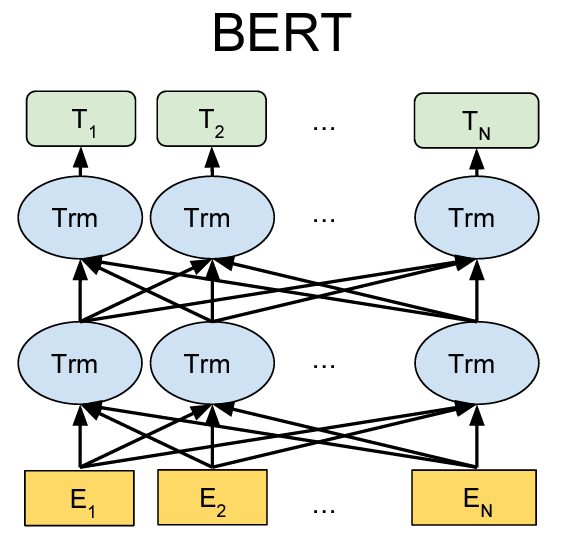
\includegraphics[width=0.3\textwidth]{figures/bert.png}
    \caption{BERT 模型结构}
    \label{fig:bert}
\end{figure}

图片引用可以使用 \verb|\figcite{}|,如:BERT 模型结构图如图 ~\ref{fig:bert}(图片来源:文献\figcite{devlin2018bert}) 所示。

\section{链接相关}
模板使用了 hyperref 包处理相关链接,使用 \verb|\href| 可以生成超链接,默认不显示链接颜色。如果需要输出网址,可以使用 \verb|\url| 命令,示例:\url{https://github.com}。